\documentclass[nobib]{tufte-handout}

%\\geometry{showframe}% for debugging purposes -- displays the margins

\newcommand{\bra}[1]{\left(#1\right)}
\usepackage{amssymb}
\usepackage{hyperref}
\usepackage[activate={true,nocompatibility},final,tracking=true,kerning=true,spacing=true,factor=1100,stretch=10,shrink=10]{microtype}
\usepackage{color}
\usepackage{steinmetz}
% Fixes captions and images being cut off
\usepackage{marginfix}
\usepackage{array}
\usepackage{tikz}
\usepackage{amsmath,amsthm}
\usetikzlibrary{shapes}
\usetikzlibrary{positioning}
\usepackage{listings}
\usepackage{caption}
\usepackage[americancurrents, americanvoltages, americanresistors, americaninductors]{circuitikz}
\DeclareCaptionFont{white}{\color{white}}
\DeclareCaptionFormat{listing}{\colorbox{gray}{\parbox{\textwidth}{#1#2#3}}}
\captionsetup[lstlisting]{format=listing,labelfont=white,textfont=white}

% Set up the images/graphics package
\usepackage{graphicx}
\setkeys{Gin}{width=\linewidth,totalheight=\textheight,keepaspectratio}
\graphicspath{{.}}

\title{ECE 20002: Electrical Engineering Fundamentals II}
\author[Zeke Ulrich]{Zeke Ulrich}
\date{\today}  % if the \date{} command is left out, the current date will be used

% The following package makes prettier tables.  We're all about the bling!
\usepackage{booktabs}

% The units package provides nice, non-stacked fractions and better spacing
% for units.
\usepackage{units}

% The fancyvrb package lets us customize the formatting of verbatim
% environments.  We use a slightly smaller font.
\usepackage{fancyvrb}
\fvset{fontsize=\normalsize}

% Small sections of multiple columns
\usepackage{multicol}

% For finite state machines 
\usetikzlibrary{automata} % Import library for drawing automata
\usetikzlibrary{positioning} % ...positioning nodes
\usetikzlibrary{arrows} % ...customizing arrows
\tikzset{node distance=2.5cm, % Minimum distance between two nodes. Change if necessary.
    every state/.style={ % Sets the properties for each state
    semithick,
    fill=gray!10},
    initial text={}, % No label on start arrow
    double distance=2pt, % Adjust appearance of accept states
    every edge/.style={ % Sets the properties for each transition
    draw,
    ->,>=stealth', % Makes edges directed with bold arrowheads
    auto,
    semithick}}
\let\epsilon\varepsilon

% These commands are used to pretty-print LaTeX commands
\newcommand{\doccmd}[1]{\texttt{\textbackslash#1}}% command name -- adds backslash automatically
\newcommand{\docopt}[1]{\ensuremath{\langle}\textrm{\textit{#1}}\ensuremath{\rangle}}% optional command argument
\newcommand{\docarg}[1]{\textrm{\textit{#1}}}% (required) command argument
\newenvironment{docspec}{\begin{quote}\noindent}{\end{quote}}% command specification environment
\newcommand{\docenv}[1]{\textsf{#1}}% environment name
\newcommand{\docpkg}[1]{\texttt{#1}}% package name
\newcommand{\doccls}[1]{\texttt{#1}}% document class name
\newcommand{\docclsopt}[1]{\texttt{#1}}% document class option name

% Define a custom command for definitions and biconditional
\newcommand{\defn}[2]{\noindent\textbf{#1}:\ #2}
\let\biconditional\leftrightarrow

% Define graphics path
\graphicspath{ {./images/} }

\tikzset{
  mirror/.code={
    \def\mirrortemp{#1} % Store the content to be mirrored
    \begin{scope}[xscale=-1] % Mirror horizontally
      \path \mirrortemp; % Draw the mirrored path
    \end{scope}
  }
}

\begin{document}

\maketitle

\begin{abstract}
    Lecture notes for Purdue's ECE 20002.
\end{abstract}

\tableofcontents

\section{Course Introduction}

Continuation of Electrical Engineering Fundamentals I. The course addresses
mathematical and computational foundations of circuit analysis (differential
equations, Laplace Transform techniques) with a focus on application to linear
circuits having variable behavior as a function of frequency, with emphasis on
filtering. Variable frequency behavior is considered for applications of
electronic components through single-transistor and operational amplifiers. The
course ends with a consideration of how circuits behave and may be modeled for
analysis at high frequencies.\\~\\ Learning Objectives:
\begin{enumerate}
    \item Analyze 2nd order linear circuits with sources and/or passive elements
    \item Compute responses of linear circuits with and without initial conditions via
          one-sided Laplace transform techniques
    \item Compute responses to linear circuits using transfer function and convolution
          techniques
    \item Analyze and design transistor amplifiers at low, mid and high frequencies
\end{enumerate}

\pagebreak

\section{Field-Effect Transistor Devices}

\subsection{MOSFETs}
Let us begin where ECE 20001 ended, with metal-oxide semiconductor 
field-effect transistors (MOSFETs). The rectangle below represent 
a wafer of silicon. The p - Si label indicates that the 
the wafer is primarily doped with boron and the primary carrier
type is holes. The two $n^+$ rectangles designate regions of phosphorus 
doping. The grey rectangles above the wafer are dielectric layers of 
silicon dioxide. The black rectangles are ohmic metals 
that allow for connecting our phosphorus regions to other components.
To these metal contacts we attach a source, a gate, and a drain.  
The source is the source of electron, and the drain is how the electrons 
exit. The gate will define a pathway between the source and drain. 
\begin{figure}
    \caption{nMOSFET diagram}
    \label{fig:nMOSFET diagram}
    \begin{center}
        \begin{circuitikz}
            \draw (0,0)
            to (4,0)
            to (4,2)
            to (0,2)
            to (0,0);
            \node at (2,1) {p - Si};
            \draw (2,0) to (2,-0.25) node[ground]{};
    
            \draw (0.5, 2) rectangle node {$n^+$} (1.5,1.5);
            \draw (2.5, 2) rectangle node {$n^+$} (3.5,1.5);
    
            \draw[fill=gray] (0,2) rectangle (0.5,2.25);
            \draw[fill=gray] (1.5,2) rectangle (2.5,2.25);
            \draw[fill=gray] (3.5,2) rectangle (4,2.25);
            
            \draw[fill=black] (0.5, 2) rectangle (1.5,2.125);
            \draw[fill=black] (1.5,2.25) rectangle (2.5,2.375);
            \draw[fill=black] (2.5, 2) rectangle (3.5,2.125);
    
            \draw (1, 2) to[short, -*] (1, 3) node[above] {Source}
            to (0.5, 3);
            \draw (2, 2.25) to[short, -*] (2, 3.25) node[above] {Gate, $v_{GS}(v_G)$};
            \draw (3, 2) to[short, -*] (3, 3) node[right] {Drain, $v_{DS}(v_D)$};
        \end{circuitikz}
    \end{center}
\end{figure}
Since the phosphorus regions are n-type and 
ergo have free electrons, the primary carrier of this MOSFET are electrons. 
The way we allow current to flow from source 
to drain is by increasing the voltage of the gate $v_{GS}$ to attract 
an inversion layer underneath the dielectric separating the gate from the 
silicon wafer. If the voltage of the gate is high enough ($v_{GS} > V_T$) then 
enough electrons will be attracted to that area for current to flow between 
source and drain. 

We could create a similar MOSFET by inverting the n-type and 
p-type regions, as in figure \ref{fig:pMOSFET}.
\begin{figure}
    \caption{pMOSFET diagram}
    \label{fig:pMOSFET}
    \begin{center}
        \begin{circuitikz}
            \draw (0,0)
            to (4,0)
            to (4,2)
            to (0,2)
            to (0,0);
            \node at (2,1) {n - Si};
            \draw (2,0) to (2,-0.25) node[ground]{};
    
            \draw (0.5, 2) rectangle node {$p^+$} (1.5,1.5);
            \draw (2.5, 2) rectangle node {$p^+$} (3.5,1.5);
    
            \draw[fill=gray] (0,2) rectangle (0.5,2.25);
            \draw[fill=gray] (1.5,2) rectangle (2.5,2.25);
            \draw[fill=gray] (3.5,2) rectangle (4,2.25);
            
            \draw[fill=black] (0.5, 2) rectangle (1.5,2.125);
            \draw[fill=black] (1.5,2.25) rectangle (2.5,2.375);
            \draw[fill=black] (2.5, 2) rectangle (3.5,2.125);
    
            \draw (1, 2) to[short, -*] (1, 3) node[above] {Source}
            to (0.5, 3);
            \draw (2, 2.25) to[short, -*] (2, 3.25) node[above] {Gate, $v_{GS}(v_G)$};
            \draw (3, 2) to[short, -*] (3, 3) node[right] {Drain, $v_{DS}(v_D)$};
        \end{circuitikz}
    \end{center}
\end{figure}
In this case the primary current carrier will be holes. 

In the case of the nMOSFET in figure \ref{fig:nMOSFET diagram}, 
a negative gate voltage will attract holes in the 
semiconductor, forming two oppositely charged areas separated 
by a distance $x$. This establishes an electric field 
within the oxide layer given by the equation for a 
parallel plate capacitor
\begin{equation} \label{eq:1}
    \mathcal{E}_x = - \frac{dV}{dx}
\end{equation}
Likewise, a positive gate voltage \emph{that is less than $V_T$} will attract electrons in the 
semiconductor. This also forms a capacitance of $C_{ox}$ in the
oxide layer, but because the semiconductor is n-type, the electrons will 
be spread out over a wider area and have their own capacitance $C_d$. 
Thus the total capacitance across the oxide and depletion region
$C$ given by
\begin{equation} \label{eq:2}
    \frac{1}{C} = \frac{1}{C_ox} + \frac{1}{C_d}
\end{equation}
If $0 < V_T < v_{GS}$, then $C=f{\omega}$, where $\omega$ is 
the frequency of our probe. 

Figure \ref{fig:p-type MOS C-V} displays the 
capacitance-voltage graph of a p-type metal-oxide 
semiconductor. The capacitance is constant when 
gate voltage is negative, then falls at the \emph{flat-band voltage}
$V_{GS} = 0V$, then rapidly rises again after the threshold voltage 
is reached. 
\begin{figure}
    \caption{p-type MOS capacitance-voltage characteristic}
    \label{fig:p-type MOS C-V}
    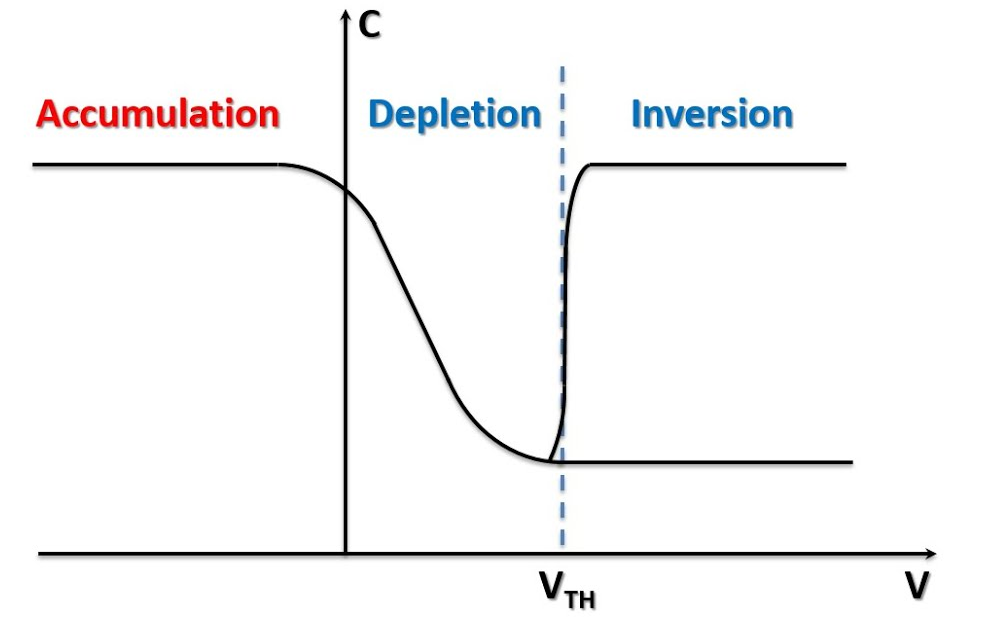
\includegraphics{moscv.png}
\end{figure}

The resistivity of the inversion channel created by the gate's bias
is given by 
\begin{equation} \label{eq:3}
    \frac{1}{\rho} = (n\mu_e + p\mu_h)q
\end{equation}
where $n$ is the concentration of electrons, 
$p$ is the concentration of holes, $\mu_e$ is
the mobility of electrons, $\mu_h$ is the 
mobility of holes, and $q$ is the charge of an electron. 
The higher the gate voltage, the higher the current between source and drain. 
Below the threshold voltage there is no current flow because no 
channel is formed. This relationship is linear provided the drain voltage 
is less than 150 mV, but above 0.3 V becomes nonlinear. That's because 
the channel is no longer a regular shape, but narrows in the region of the 
drain. Below 150 mV, however, this distortion can be assumed negligible. 
Recall that 
\begin{equation} \label{4}
    R = \frac{\rho L}{A}
\end{equation}
Whereas for small $v_{DS}$ the area is almost constant, 
when $v_{DS} > 0.15 V$ the area $A$ decreases enough that 
the resistance $R$ is significantly increased. When the area has 
decreased to zero at the drain, we reach the \emph{pinch-off} and 
the drain voltage is at saturation $v_{DS(sat)}$. The current still 
flows constantly for all drain voltage above saturation, however. 
Before saturation is reached and after the gate voltage is above the threshold, 
we are in the triode region. In the triode region, the current is given by 
\begin{equation} \label{eq:5}
    i_{D(triode)} = \mu C_{ox} \frac{W}{L} ((v_{GS}-V_T)v_{DS}-\frac{v^2_{DS}}{2})
\end{equation}
Sometimes, the constant terms are wrapped up into 
one constant, like so:
\begin{equation} \label{eq:6}
    i_{D(triode)} = k_n ((v_{GS}-V_T)v_{DS}-\frac{v^2_{DS}}{2})
\end{equation}
In the saturation region, 
\begin{align} \label{eq:7}
    i_{D(sat)} &= \mu C_{ox} \frac{W}{L} \frac{(v_{GS}-V_T)^2}{2} \\
    &= k_n \frac{v^2_{DS(sat)}}{2}
\end{align}
When we are far away from saturation, 
the resistance of the channel is given by 
\begin{align} \label{eq:8}
    R_{on} &= \frac{\partial v_{DS}}{\partial i_D} \\
    &= \frac{1}{\mu C_{ox} \frac{W}{L} (v_{GS} - V_T)}
\end{align}

Figure \ref{fig:Transfer Characteristics} shows a family of $i_D$-$v_{DS}$
curves with differing values of $v_{GS}$. 
\begin{figure}
    \caption{Transfer characteristics of nMOSFETs}
    \label{fig:Transfer Characteristics}
    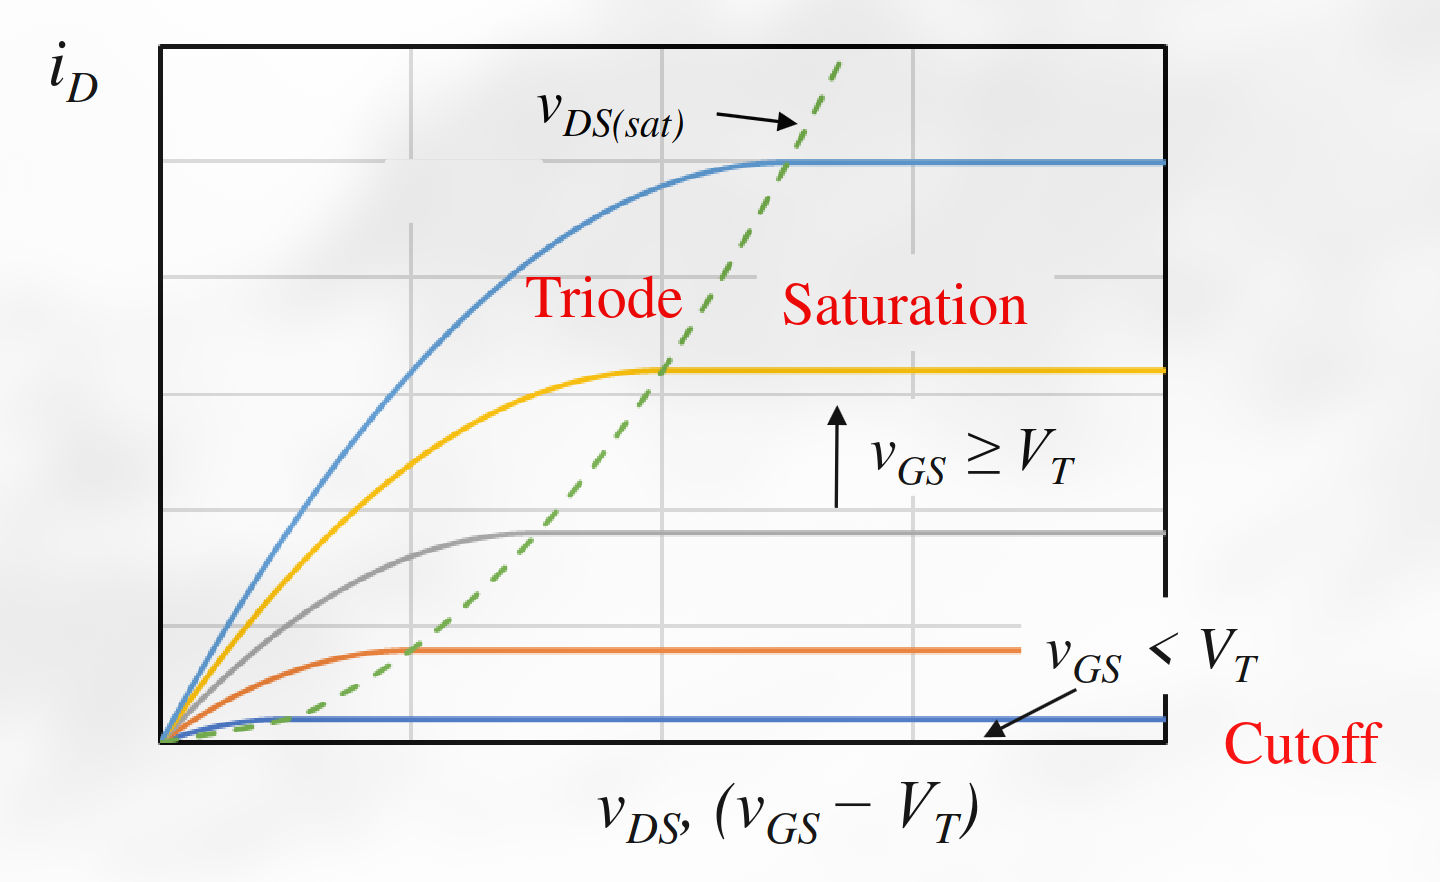
\includegraphics{Transfer Characteristics.png}
\end{figure}
Also show as a dashed green line is the saturation current 
as a function of gate voltage. Let's look at the impact 
the threshold voltage has by plotting the $i_D$-$v_{GS}$ curve 
for differing values of $V_T$ in figure \ref{fig:idvgsvt}. 
\begin{figure}
    \caption{$i_D$-$v_{GS}$ curve for select values of $V_T$}
    \label{fig:idvgsvt}
    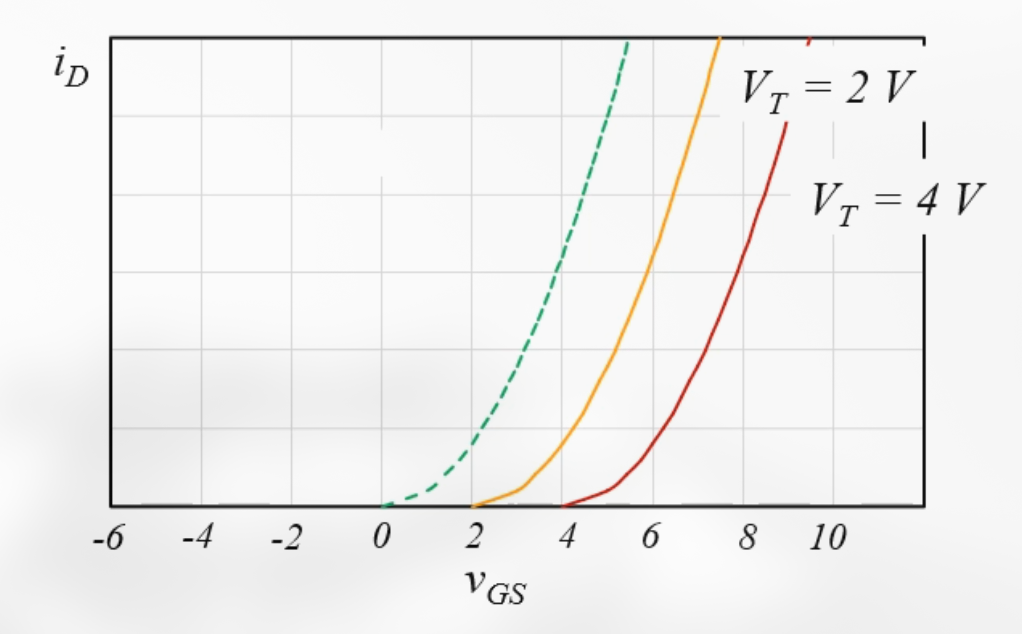
\includegraphics{idvgsvt.png}
\end{figure}
Now the green dashed curve corresponds to a threshold voltage of zero. 
Recall that the threshold voltage is intrinsic to 
the semiconductor wafer. Doping variations, defect, and shape can 
all affect the threshold voltage. If we build a depletion-mode nMOSFET,
then we allow for negative threshold voltages.

A normally off like in figure \ref{fig:nMOSFET diagram} 
has the symbol shown in \ref{fig:nMOSFET schematic} and 
is said to be in enhancement mode. 
\begin{figure}
    \caption{nMOSFET schematic}
    \label{fig:nMOSFET schematic}
    \begin{center}
        \begin{circuitikz}
            \draw (0,0) node[nmos] (mosfet) {};
            \draw (mosfet.D) -- ++(0,-0.5) node[right] {$V_{D}$};
            \draw (mosfet.S) -- ++(0,-0.1) node[right] {$V_S$}
            -- ++(0, 0.6) 
            -- ++(-0.5,0)
            to[short, i=~] ++(0.5,0);
            \draw (mosfet.G) -- ++(-0.5,0) node[left] {$V_{GS}$};
        \end{circuitikz}
    \end{center}
\end{figure}
If the nMOSFET has an n-channel between the source and 
drain, as shown in figure \ref{fig:nMOSFET diagram on}, 
\begin{figure}
    \caption{ Normally on nMOSFET diagram}
    \label{fig:nMOSFET diagram on}
    \begin{center}
        \begin{circuitikz}
            \draw (0,0)
            to (4,0)
            to (4,2)
            to (0,2)
            to (0,0);
            \node at (2,1) {p - Si};
            \draw (2,0) to (2,-0.25) node[ground]{};
    
            \draw (0.5, 2) rectangle node {$n^+$} (1.5,1.65);
            \draw (2.5, 2) rectangle node {$n^+$} (3.5,1.65);
    
            \draw[fill=gray] (0,2) rectangle (0.5,2.25);
            \draw[fill=gray] (1.5,2) rectangle (2.5,2.25);
            \draw[fill=gray] (3.5,2) rectangle (4,2.25);
            
            \draw[fill=black] (0.5, 2) rectangle (1.5,2.125);
            \draw[fill=black] (1.5,2.25) rectangle (2.5,2.375);
            \draw[fill=black] (2.5, 2) rectangle (3.5,2.125);
    
            \draw (1, 2) to[short, -*] (1, 3) node[above] {Source}
            to (0.5, 3);
            \draw (2, 2.25) to[short, -*] (2, 3.25) node[above] {Gate, $v_{GS}(v_G)$};
            \draw (3, 2) to[short, -*] (3, 3) node[right] {Drain, $v_{DS}(v_D)$};

            \draw[fill=green] (1.5, 2) rectangle (2.5, 1.75) node[below] {n-channel}; 
        \end{circuitikz}
    \end{center}
\end{figure}
then it is normally on and its symbol is as seen in 
figure \ref{fig:nMOSFET on schematic}. This kind of nMOSFET 
is said to be in depletion mode. 
\begin{figure}
    \caption{Schematic of normally on nMOSFET}
    \label{fig:nMOSFET on schematic}
    \begin{center}
        \begin{circuitikz}
            \draw (0,0) node[nmosd] (mosfet) {};
            \draw (mosfet.D) -- ++(0,-0.5) node[right] {$V_{D}$};
            \draw (mosfet.S) -- ++(0,-0.1) node[right] {$V_S$}
            -- ++(0, 0.6) 
            -- ++(-0.5,0)
            to[short, i=~] ++(0.5,0);
            \draw (mosfet.G) -- ++(-0.5,0) node[left] {$V_{GS}$};
        \end{circuitikz}
    \end{center}
\end{figure}
Note the thicker line between source and drain representing 
the n-channel. 

Similarly, the pMOSFET shown in figure \ref{fig:pMOSFET} is 
a normally off, enhancement mode pMOSFET. A pMOSFET with a 
p-channel is normally on and in depletion mode. 

Let's look at the transfer characteristics of 
the different types of MOSFETs. figure \ref{fig:Transfer Characteristics} 
shows these characteristics for a normally off, enhancement mode 
nMOSFET.
For a normally on, depletion mode nMOSFET the graph is exactly 
the same, except that the current can flow even when the 
gate bias is zero since the fabricated channel allows 
the flow of electrons from source to drain.
The output characteristics for a normally off, enhancement mode pMOSFET
are shown in figure \ref{fig:idvgsvt pmosfet}.
\begin{figure}
    \caption{$i_D$-$v_{DS}$ curve for select values of $v_{GS}-V_T$}
    \label{fig:idvgsvt pmosfet}
    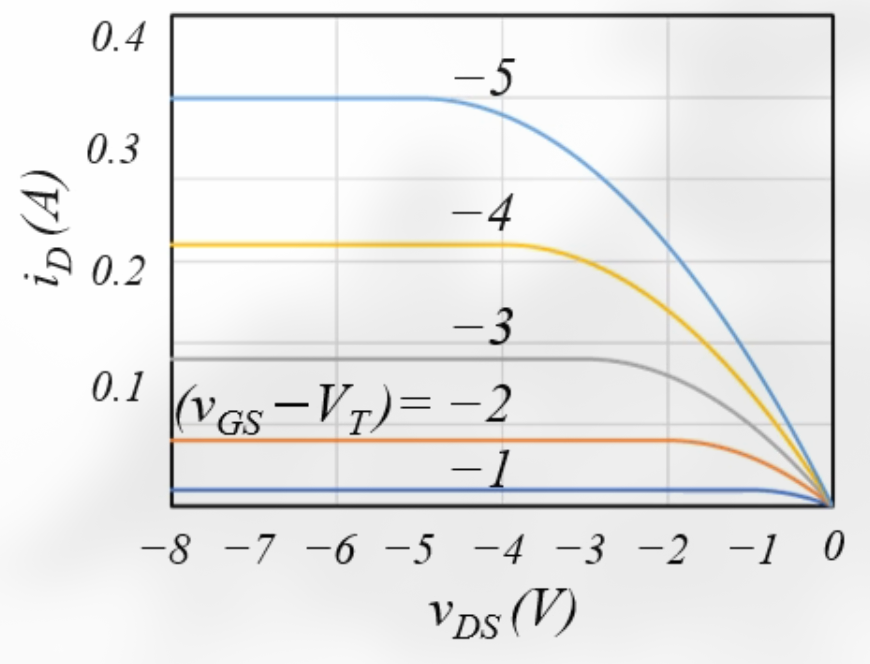
\includegraphics{output characteristics pmosfet.png}
\end{figure}
A negative bias on the gate will induce a channel of positive holes 
in the semiconductor, making the threshold voltage for a pMOSFET 
negative. Again, the normally on depletion mode pMOSFET graph has the same 
shape, but since there is an existing channel for current it will flow even for 
some positive values of $v_{GS}$. We need to deplete the channel by pushing away all 
the holes in it with the bias on the gate in order to turn it off. 

To review, there for four kinds of MOSFETs in which we are interested:
\begin{itemize}
    \item normally off, enhancement mode nMOSFETs
    \item normally on, depletion mode nMOSFETs
    \item normally off, enhancement mode pMOSFETs
    \item normally on, depletion mode pMOSFETs
\end{itemize}

\subsection{Transconductance}

Now, let us move on the the topic of transconductance. 
In the triode region, the transconductance is defined as 
\begin{equation} \label{eq:9}
    g_m = \frac{i_D}{v_{GS}} \rvert_{Q_{pt}}
\end{equation}
where 
\begin{equation}
    Q_{pt} = (I_D, V_{DS}).
\end{equation}
If we recall equation \ref{eq:5}, and substitute
for $i_D$ in equation \ref{eq:9}, then we obtain 
\begin{align}
    g_m &= \mu C_{ox} \frac{W}{L} v_{DS} \\
    &= \frac{i_{D(triode)}}{(v_{GS}-v_T)-\frac{v_{DS}}{2}}
\end{align}

In the saturation region, 
\begin{equation} \label{eq:10}
    g_m = \frac{di_D}{dv_{GS}} \rvert_{Q_{pt}}
\end{equation}
and 
\begin{equation} \label{eq:11}
    i_{D(sat)} = \mu C_{ox} \frac{W}{L} \frac{(v_{GS}-V_T)^2}{2}.
\end{equation}
Again combining these two equations, 
\begin{align} \label{eq:12}
    g_m &= \mu C_{ox} \frac{W}{L}(v_{GS} - V_T) \\
    &= \frac{2i_{D(sat)}}{(v_{GS}-V_T)}
\end{align}
The larger the transconductance, the larger 
the gain of an amplifier circuit 
that uses the transistor. 

\subsection{Channel length modulation}

By adjusting the voltage of the drain, we 
can modulate the channel length. Specifically, 
\begin{align} \label{eq:13}
    i_{D(sat)} &\propto \frac{1}{L-\Delta L} \\
    &\equiv \frac{1}{L}\left(1 + \frac{\Delta L}{L}\right).
\end{align}
And 
\begin{equation} \label{eq:14}
    \Delta L \propto (v_{DS} - v_{DS(sat)})
\end{equation}
means that 
\begin{equation} \label{eq:15}
    i_{D(sat)} = \frac{1}{2} \mu C_{ox} \frac{W}{L} (v_{GS}-V_T)^2 \left[1 + \lambda(v_{DS}-v_{DS(sat)})\right]
\end{equation}
where $\lambda$ is the empirically determined 
channel length modulation parameter. 
The output resistance at the drain is given by 
\begin{align} \label{eq:16}
    r_0 &= \left[\frac{\partial i_{D(sat)}}{\partial v_{DS}}\right]^{-1} \\
    &= \left[\lambda \frac{1}{2} k_n (v_{GS}-V_T)^2\right]^{-1} \\
    &= \frac{1}{\lambda I_{D(sat)}} \\
    &\approx \frac{V_A}{I_{D(sat)}}
\end{align}
Channel length modulation is not important when 
channel length is relatively large, but it is important 
on modern transistors where are on the order of nanometers. 

\subsection{MOSFETs in DC circuits}
Consider a circuit with two enhancement mode pMOSFETs. 
\begin{figure}
    \caption{MOSFET DC circuit}
    \label{fig:MOSFET DC circuit 1}
    \begin{center}
        \begin{circuitikz}
            \draw (0,0) node[nmos, left, xscale=-1] (m1) {};
            \node at (0,0) {$M_1$};
            \draw (m1.D) to ++(1,0);
            \draw[->] (m1.D) to ++(0,-0.25);
    
            \draw (2,0) node[nmos, left] (m2) {};
            \node at (2,0) {$M_2$};
            \draw[->] (m2.D) to ++(0,-0.25);
            \draw (m2.D) to ++(-1,0)
            to[short, -o] ++(0, 0.5) node[above] {$V^+$};
    
            \draw (m2.S) to[short, i=$I_{OUT}$] ++(0,-1);
            \draw (m2.G) to ++(0, -0.75)
            to (m1.S)
            to[R, i=$I_{REF}$, l=$R_{REF}$] ++(0,-1.5) node[ground] {};
        \end{circuitikz}
    \end{center}
\end{figure}
Notice that in figure \ref{fig:MOSFET DC circuit 1}, 
the drain of $M_1$ is directly attached to the gate. From 
this we have 
\begin{align} \label{eq:17}
    v_{DS1} &= v_{GS1} \\
    &= v_{GS2}
\end{align}
We are told $M_1$ is in saturation. If these are two identical 
transistors, then 
\begin{align} \label{eq:18}
    I_{REF} &= I_{D(sat)} \\
    &= \frac{1}{2} k_{p1} (v_{GS1} - V_{T1})^2\\
    &= I_{OUT}.
\end{align}
From this, we learn that the reference current 
is mirrored by the drain current if 
$k_{p1} = k_{p2}$ and $v_{GS1} = v_{GS2}$. 

Let us now look at the inverter shown in figure \ref{fig:MOSFET DC circuit 2}. 
\begin{figure}
    \caption{Inverter}
    \label{fig:MOSFET DC circuit 2}
    \begin{center}
        \begin{circuitikz}
            \draw (0,0) node[pmos, left] (m2) {};
            \node at (0,0) {$M_2$};
            \draw[->] (m1.D) to ++(0,-0.25);
            \draw (m2.D) to ++(0,-0.25);
            \node[left] at (m2.D) {$D_2$};
            \node[left] at (m2.S) {$S_2$};

            \draw[short, -o] (0,0.5) to ++(0, 1) node[above] {$5V$};
    
            \draw (0,-2) node[nmos, left] (m1) {};
            \node at (0,-2) {$M_1$};
            \node[left] at (m1.S) {$S_1$};
            \node[left] at (m1.D) {$D_1$};

            \draw (m1.D) to ++(0,0.25)
            to[short, -o] ++(0.5,0) node[right] {$V_{out}$};

            \draw[->] (m1.S) to ++(0,-0.125);
            \draw (0, -3) to[R] ++(0,-1) node[ground] {};

            \draw (m1.G) to ++(0,1);
            \draw (m2.G) to ++(0,-1)
            to[short, -o] ++(-1, 0) node[above] {$V_{in}$} node[below] {G};
        \end{circuitikz}
    \end{center}
\end{figure}
Let's try to find $V_{out}$ for $V_{in} = 0V$ and $V_{in} = 5V$. 
We are told that $V_{T(M1)} = 1V$ and $V_{T(M2)} = -1V$, because 
M1 is an enhancement mode nMOSFET and M2 is an enhancement mode 
pMOSFET. When $V_{in} = 0V$, M1 is off because $v_{GS1} < V_{T(M1)}$. 
Likewise, M2 is on because $v_{GS2} < V_{T(M2)}$ (recall that M2 is a pMOSFET).  
Since M1 is off, no current flows and $V_{out} = 5V$. For $V_{in} = 5V$, 
M1 flips on while M2 is off. Since M2 is off, no current flows. 
That means that $V_{out} = 5V$.

\subsection{Transistors as amplifiers}
The circuit shown in figure \ref{fig:Transistor as amplifier}
\begin{figure}
    \caption{Common-source nMOSFET amplifier circuit}
    \label{fig:Transistor as amplifier}
    \begin{center}
        \begin{circuitikz}
            \draw (0,0) node[nmos, left] (mos) {}
            (mos.G) to ++(-1,0)
            to[V, l=$v_{gs}$] ++(0,-1)
            to[V, l=$V_{GS}$] ++(0,-1)
            node[left] {$3.5 V$}
            to ++(2, 0)
            node[ground] {}
            to (mos.S);

            \node at (0, 3.2) {$V_{DD} = +10V$};
            \draw (0, 3) to[R, i=$i_D$, l=$R_D: 3.3k \Omega$, o-] (mos.D);
        \end{circuitikz}
    \end{center}
\end{figure}
has both AC and DC voltage sources. The source labelled 
by $V_{GS}$, all caps, is the DC voltage. The source 
$v_{gs}$, all lowercase, is the AC. This is not to be 
confused with $v_{GS}$, the total gate bias. The mix of 
cases indicates we have both AC and DC bias in consideration. 
The cool thing about this circuit is a small oscillation in 
the AC input induces a much larger oscillation in the 
output, hence calling it an amplifier. The output signal 
is going to be phase shifted by $180^\circ$. We can calculate the gain 
with eq. \ref{eq:19}
\begin{equation} \label{eq:19}
    A_v = \frac{v_{ds}}{v_{gs}}
\end{equation}
In this instance, 
\begin{align} \label{eq:20}
    A_v &= \frac{v_{ds}}{v_{gs}} \\
    &= \frac{4.17\angle 180^\circ}{1\angle 0^\circ} \\
    &= -4.17
\end{align}
This gain, however, will be somewhat distorted. To reduce distortion 
we need that $\lvert v_{gs} \rvert <<2(V_{GS}-V_T)$. The exact value 
of the "much less" symbol $<<$ will depend on the application, 
but it's common to require $\lvert v_{gs} \rvert < 0.2(V_{GS} - V_T)$. 
If we assume the small signal condition and no channel length modulation, then the transconductance
of the amplifier is 
\begin{equation} \label{eq:21}
    g_m = \sqrt{2k_n I_{D(sat)}}
\end{equation}

\subsection{Common-source amplifier circuit}

Figure \ref{fig:cs amplifier} shows the small signal equivalent circuit
of a common source amplifier. 
\begin{figure}
    \begin{center}
        \begin{circuitikz}
            \draw (4,-1) node[nmos] (mosfet) {};
            \draw (mosfet.S) -- ++(0,-0.1)
            -- ++(0, 0.6) 
            -- ++(-0.5,0)
            to[short, i=~] ++(0.5,0);

            \draw (0,0) to[V, invert, l=$V_{DD}$] ++(0,2)
            -- ++(4,0)
            to[R, i=$i_D$, l=$R_D$] (mosfet.D)
            ;
            \draw (mosfet.D) to[short, -o] ++(1,0) node[below] {$+$};
            \draw (mosfet.S) to ++(0,-1.25)
            to[short, -o] ++(1,0) node[above] {$-$}
            -- ++(-5, 0)
            -- ++(0,3);

            \node at (5, -1.5) {$v_{DS}$};

            \draw (mosfet.G) -- ++(-1,0)
            to[sV, l=$v_g$] ++(0, -1)
            to[V, l=$V_{GS}$] ++(0,-1)
            node[ground] {};
        \end{circuitikz}
    \end{center}
    \caption{Small signal equivalent circuit}
    \label{fig:cs amplifier}
\end{figure}
Notice the two voltage sources, one AC signal 
and one DC bias at the gate. The total 
input signal is given by
\begin{align} \label{eq:22}
    v_{GS}(t) &= v_{gs}(t) + V_{GS} \\
    v_{DS}(t) &= v_{ds}(t) + V_{DS}
\end{align}
The drain current for such a circuit 
when channel length modulation is accounted for 
is given by 
\begin{align*} \label{eq:23}
    i_{D(clm)} = \frac{1}{2}k_n \left[ v^2_{gs} + 2(V_{GS} - V_T)v_{gs} + (V_{GS} - V_T)^2 \right] \\
    \times \left[ 1 + \lambda(V_{DS} - (V_{GS} - V_T)) + \lambda(v_{ds} - v_{gs}) \right]
\end{align*}
When channel length modulation can 
be ignored, the current reduces to 
\begin{equation} \label{eq:24}
    i_{D(sat)} = \frac{1}{2}k_n \left[ v^2_{gs} + 2(V_{GS} - V_T)v_{gs} + (V_{GS} - V_T)^2 \right]
\end{equation}
For finite output resistance $r_0$, 
\begin{align} \label{eq:25}
    \frac{1}{r_0} &= \left[ \frac{\partial i_{D(clm)}}{\partial v_{DS}} \right] \\
    &= \frac{\partial}{\partial v_{DS}} \left\{ \frac{k_n}{2} (v_{GS} - V_T)^2 \left[ 1 + \lambda(v_{DS} - v_{DS(sat)}) \right] \right\} \\
    &= \frac{k_n}{2} (v_{GS} - V_T)^2 \frac{\partial}{\partial v_{DS}} \left[ 1 + \lambda(v_{DS} - v_{DS(sat)}) \right] \\
    &= \lambda \frac{k_n}{2} (v_{GS} - V_T)^2 \\
    &= \lambda I_{D(sat)}.
\end{align}
We then define the \emph{intrinsic voltage gain of a MOSFET}
as 
\begin{align}
    \mu_f &= g_m r_0 \\
    &= \sqrt{2k_n I_{D(sat)}} \left( \frac{1}{\lambda I_{D(sat)}} \right) \\
    &= \frac{1}{\lambda} \sqrt{\frac{2k_n}{I_{D(sat)}}}
\end{align}
We can greatly simplify circuit analysis 
by breaking the circuit up into 
AC and DC. To find the DC equivalent 
circuit, follow these steps: 
\begin{enumerate}
    \item Replace all capacitors with open circuits
    \item Replace all inductors with short circuits
    \item Deactivate AC sources 
    \item Find the Q-point using the DC equivalent circuit
\end{enumerate}
To find the AC equivalent circuit, 
\begin{enumerate}
    \item Replace all capacitors with short circuits at operational frequency
    \item Replace all inductors with open circuits at operational frequency
    \item Deactivate DC voltages and replace with short circuits 
    \item Deactivate DC current sources and replace with open circuits 
    \item Replace the transistor with its small-signal model 
\end{enumerate}


\subsection{Chapter summary}

\begin{figure}
    \begin{center}
        \begin{tabular}{ c | c }
            Region & Conditions \\
            \hline
            Cut-off & $v_{GS} < V_T$ \\
            Triode & $v_{DS} > v_{DS(sat)}$\\
            Saturation & $v_{DS} \leq v_{DS(sat)}$\\
            \hline
        \end{tabular}
    \end{center}
    \caption{nMOSFET regions of operation}
    \label{tab:nMOSFET regions}
\end{figure}

\begin{figure}
    \begin{center}
        \begin{tabular}{ c | c }
            Region & Conditions \\
            \hline
            Cut-off & $v_{GS} > V_T$ \\
            Triode & $v_{DS} \leq v_{DS(sat)}$\\
            Saturation & $v_{DS} > v_{DS(sat)}$\\
            \hline
        \end{tabular}
    \end{center}
    \caption{pMOSFET regions of operation}
    \label{tab:pMOSFET regions}
\end{figure}

\begin{figure}
    \begin{center}
        \begin{tabular}{ c | c | c }
            & nMOSFET & pMOSFET \\
            \hline
            Cutoff & $v_{GS} < 0$ & $v_{GS} > 0$ \\
            Triode & $v_{GS} > 0$ & $v_{GS} < 0$ \\
            Saturation & $v_{GS} > 0$ & $v_{GS} < 0$ \\
            \hline
            Enhancement & $V_T > 0$ & $V_T < 0$ \\
            Depletion & $V_T < 0$ & $V_T > 0$ \\
            \hline
        \end{tabular}
    \end{center}
    \caption{Differences between pMOSFET and nMOSFET}
    \label{tab:pn differences}
\end{figure}

\begin{figure}
    \begin{center}
        \begin{tabular}{ c | c | c }
             & nMOSFET & pMOSFET \\
            \hline 
            Enhancement &
            \begin{circuitikz}
                \draw (0,0) node[nmos] (mosfet) {};
                \draw (mosfet.D) -- ++(0,-0.5) node[right] {$V_{D}$};
                \draw (mosfet.S) -- ++(0,-0.1) node[right] {$V_S$}
                -- ++(0, 0.6) 
                -- ++(-0.5,0)
                to[short, i=~] ++(0.5,0);
                \draw (mosfet.G) -- ++(-0.5,0) node[left] {$V_{GS}$};
            \end{circuitikz}
            & 
            \begin{circuitikz}
                \draw (0,0) node[pmos] (mosfet) {};
                \draw (mosfet.D) -- ++(0,-0.25) node[right] {$V_{D}$};
                \draw (mosfet.S) -- ++(0,0.1) node[right] {$V_S$}
                -- ++(0, -0.6) 
                to[short, i=~] ++(-0.5,0);
                \draw (mosfet.G) -- ++(-0.5,0) node[left] {$V_{GS}$};
            \end{circuitikz}
            \\
            \hline 
            Depletion & 
            \begin{circuitikz}
                \draw (0,0) node[nmosd] (mosfet) {};
                \draw (mosfet.D) -- ++(0,-0.5) node[right] {$V_{D}$};
                \draw (mosfet.S) -- ++(0,-0.1) node[right] {$V_S$}
                -- ++(0, 0.6) 
                -- ++(-0.5,0)
                to[short, i=~] ++(0.5,0);
                \draw (mosfet.G) -- ++(-0.5,0) node[left] {$V_{GS}$};
            \end{circuitikz} 
            & 
            \begin{circuitikz}
                \draw (0,0) node[pmosd] (mosfet) {};
                \draw (mosfet.D) -- ++(0,-0.25) node[right] {$V_{D}$};
                \draw (mosfet.S) -- ++(0,0.1) node[right] {$V_S$}
                -- ++(0, -0.6) 
                to[short, i=~] ++(-0.5,0);
                \draw (mosfet.G) -- ++(-0.5,0) node[left] {$V_{GS}$};
            \end{circuitikz} 
            \\
        \end{tabular}
    \end{center}
    \caption{MOSFET schema}
    \label{tab:MOSFET schema}
\end{figure}

\begin{center}
    \begin{tabular}{ c | c }
        Equation & Reference \\
        \hline
        $v_{DS(sat)} = v_{GS} - V_T$ \\
        \hline
        $i_{D(cutoff)} = 0$ & \\
        \hline
        $i_{D(triode)} = \mu C_{ox} \frac{W}{L} ((v_{GS}-V_T)v_{DS}-\frac{v^2_{DS}}{2})$ \\
        $= k_n ((v_{GS}-V_T)v_{DS}-\frac{v^2_{DS}}{2})$
        & eq. \ref{eq:5} \\
        \hline
        $i_{D(sat)} = \mu C_{ox} \frac{W}{L} \frac{(v_{GS}-V_T)^2}{2}$ \\
        $= k_n \frac{v^2_{DS(sat)}}{2}$
        & eq. \ref{eq:7} \\
        \hline
    \end{tabular}
\end{center}

\end{document}
